\documentclass{article}
\usepackage[utf8]{inputenc}
\usepackage{graphicx}

\title{Eye and Vision}
\author{MCB C61 with Professor David Presti \\ \\ Benjamin Lee}
% \date{15 March 2018}

\begin{document}

\maketitle

\textbf{Key Concepts:}
\begin{itemize}
    \item Electromagnetic Spectrum, visible light
    \item Retina
    \item Fovea
    \item Blind Spot
    \item Photoreceptor Cells: rods, cones
    \item Retinal achromatopsia
    \item Photoreceptor cells: inner and outer segments
    \item Retinal, retinol (vitamin A), beta-carotene
    \item Photoisomerization of retinal(cis to trans) \item GPCR intracellular cascade
    \item Retina: bipolar cells, ganglion cells
    \item Retina: horizontal cells, amacrine cells
    \item Receptive field
    \item Visual map: world to retina to cortex
    \item LGN, visual cortex (V1 etc)
    \item Superior Colliculus
    \item Scotoma, hemianopia
    \item Cortical achromatopsia
    \item Motion blindness 
    \item Prosopagnosia
    \item Agnosia
\end{itemize}

\newpage
\section{Electromagnetic Spectrum}
Our visual system responds to electromagnetic radiation in the energy range called \textbf{visible light}. \\

\noindent Electromagnetic energy can be conceptualized as a \textbf{vibrating electromagnetic field} moving/radiating through space. Described quantitatively as either a frequency or vibration (in cycles per second, or herts) or wavelength in meters. \\

\noindent Can also be conceptualized as \textbf{packets of energy}, called photons. \\

\noindent Description of light and other electromagnetic energy as simultaneously\textbf{ both a wavelike field and particle-like photons} is profound and was central to the development of quantum physics in the early 20th century. 

\begin{itemize}
    \item Visible light energy range between 400-700 nanometers (nm) 
    \item Range of energy can engage in significant and sustainable (nondamaging) interactions with molecular and cellular structures in the body. 
    \item Radiation is more \textbf{energetic (shorter wavelength)} than visible light: ultraviolet, x-ray, and gamma-ray regions of the spectrum 
        \subitem Interactions with molecular and cellular structures likely to be damaging
        \subitem Break chemical bonds, free radicals form, DNA damaged, cell membranes leaky, etc. 
    \item Radiation is \textbf{lower in energy (longer wavelength)} than visible light: infrared, microwave, and radio wave regions of the spectrum 
        \subitem Interaction with molecular and cellular structures might not be energetic enough to generate a reliable neural signal
\end{itemize}

\newpage
\section{Eyeballs}
Receptive organ for human vision. Analogous to the camera in that in a camera a lens focuses incoming light onto a photosensitive film or detector. \\
The cornea, lens and pupil focus light onto the photosensitive retina at the rear of the eyeball. \\

\begin{figure}[htp]
\centering
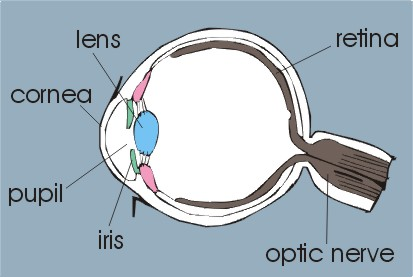
\includegraphics[width=6cm]{images/eyeball.jpg}
\caption{Eyeball}
\label{fig: eyeball}
\end{figure}

\textbf{Retina:} Complex structure, consisting of a layer of light-sensitive photoreceptor cells and several layers of interconnected nerve cells. \\
\textit{Retina} derives from Latin \textit{rete}, meaning "net", referring to the complex network of cell bodies, nerve fibers and blood vessels that compose it. \\

\textbf{Fovea:} Density of photoreceptors is highest here because light is focused here by the cornea and the lens. So visual acuity (ability to see fine detail) is best for the region we are looking at. \\
Latin for "pit". \\

\begin{figure}[htp]
\centering
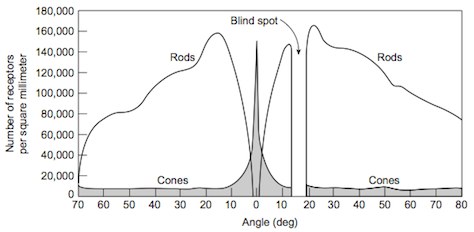
\includegraphics[width=10cm]{images/RodConeDensity.png}
\caption{Photoreceptor Density Graph}
\label{fig: Density graph}
\end{figure}

\textbf{Two major photoreceptor cells:}
\begin{itemize}
    \item \textbf{Rods:} rod shaped, numerous, distributed throughout most of the retina, and sensitive to small amounts of light. 
    \item \textbf{Cones:} cone shaped, mostly located in fovea, responds to higher intensity rather than dim light. 
    \item 3 Different types of cone cells:
        \subitem Short-wavelength(S) (Blue)
        \subitem Medium-wavelength(M) (Green)
        \subitem Longer-wavelength(L) (Red)
    \item Rod and cone cells contain specific protein molecules called \textit{rhodopsin} and \textit{cone opsins} 
        \subitem Absorb light and initiate the process of transformation of the light energy into a neural signal. Also absorb different regions of the visible light spectrum. 
\end{itemize}

\begin{figure}[htp]
\centering
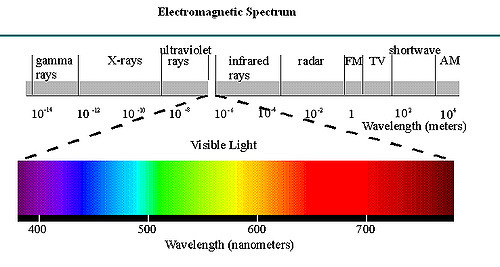
\includegraphics[width=9cm]{images/electro2.jpg}
\caption{Electromagnetic Spectrum}
\label{fig: Electro Spectrum}
\end{figure}

As the wavelength moves from 400nm-700nm, we perceive a rainbow of colors: violet, blue, green, yellow, orange, and red. Colors don't exist "out there". It's just how our minds perceive it. \\
\indent Some animals have two cone photoreceptor types; dichromatic color vision, less rich visual experience of color \\
\indent Many birds have tetrachromatic color vision: four different cone types, more discriminate of wavelengths and richer color experience. \\

\textbf{Retinal Achromatopsia:} genetic or developmental anomaly results in loss of all functional cone cells. No experience of color, only see in shades of black, white, and gray. \\
People with retinal achomatopsia report seeing more subtle gradations of contrast, shadow and texture than someone with normal vision. \\

\textbf{Blind Spot:} The place where the axons from the neurons in the retina come together into a bundle called the optic nerve and exit the eyeball on the way to the brain. There are no photoreceptors here at all. (about one million nerve fibers occupy it)\\
Although we are completely blind in that region, we are unaware the blindness. Why? Because each of our eyes have different blind spot areas, so one eye can make up for the other eyes blind spot, our visual system also makes up for the blind spot with information because we are constantly moving, and even if we keep our head still we only notice it when we bring our attention to it because it has been with us our entire evolution, so our system has to have made up for it. \\

\subsection{Photoreceptor cells: inner and outer segments}

\textbf{Rod:}
\begin{itemize}
    \item \textbf{Outer:} Rodlike segment containing numerous lipid bilayer membrane disks, each disk containing numerous \textit{rhodopsin} photoreceptor proteins embedded in the disks. 
    \item Each rod cell contains 10$^8$ or one hundred million rhodopsin molecules
    \item There are one hundred million rod cells in a rentina, so about 10$^16$ (ten quadrillion) rhodopsin molecules in each of our two retinas
    \item \textbf{Inner:} Contains the nuclei, mitochondria, and other structures necessary for the functioning of the cell. 
\end{itemize}

\textbf{Cone:}
\begin{itemize}
    \item \textbf{Outer:} Cone-shaped segment containing cone \textit{opsin} photoreceptor proteins embedded in a highly infolded cell membrane
    \item \textbf{Inner:} Contains the nuclei, mitochondria, and other structures necessary for the functioning of the cell. 
\end{itemize}

Each rhodopsin or cone opsin protein is composed of about 350 amino acids joined into a long chain by covalent chemical bonds. The chain is embedded in lipid bilayer membrane in the \textit{outer segment} of a photoreceptor cell. Winds itself back and forth across the bilayer \textbf{seven times}. Where the polypeptide chain crosses the membrane, it forms alpha-helical structures composed of amino acids that are more hydrophobic and thus agreeable to being inside the hydrophobic core of the lipid bilayer. \\

\subsection{Retinal}
\textbf{Retinal:} The small molecule in a rhodopsin or cone opsin attached to the opsin protein via a covalent bond with a nitrogen atom in a specific lysine amino acid within the protein. \\
\textbf{Absorbs} the light and begins the cascade of events leading to a neural signal. \\

\noindent Our body cannot make retinal from scratch. Must eat \underline{Vitamin A} and \underline{carotenoids}. \\

\noindent \textbf{Retinol:} also known as Vitamin A, differs from retinal by the addition of hydrogen to the oxygen atom at the end of the chain (converting the aldehyde to an alcohol). \\
\textbf{Carotenoids:} beta-carotene for example, widespread in plants and are the most abundant chemical precursors to retinal and retinol in nature. (Beta-carotene gives carrots their orange color) \\

Our body knows how to take beta-carotene, cleave it half, and chemically modify it to yield two molecules of retinal. 

\subsubsection{Photoisomerization (light-induced isomerization):} 
\begin{itemize}
    \item When the retinal molecule is bound to the protein in rhodopsin or one of the cone opsins, it occurs in a form called the \textbf{11-\textit{cis}} isomer of retinal (carbon-chain bent or kinked)
    \item Absorption of a photon of light by the retinal molecule triggers a change in the shape of the chain so that it rotates around the double bond where the kink is and straightens out, into a form called the \textbf{all-\textit{trans}} isomer of retinal
\end{itemize}

\begin{figure}[htp]
\centering
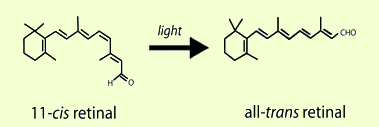
\includegraphics[width=6cm]{images/CistoTrans.png}
\caption{11-cis-retinal to all-trans-retinal}
\label{fig: cis to trans}
\end{figure}

This straightening causes the retinal to push on amino acids surrounding it and shapes the entire opsin protein into what we know as GPCRs (G-protein coupled proteins) 

\subsubsection{GPCR intracellular cascade}
When they shape change, a cascade of intracellular event is initiated. \\
Neuronal signaling at synapses, the binding of a neurotransmitter molecule shape-shifted the GPCR; here, the light-induced isomerization of the retinal changes the shape. \\
Opsin GPCRs are light detectors \\

\noindent \textbf{Rhodopsin GPCR cascade:}
\begin{itemize}
    \item Photon of light is absorbed by the by \textbf{11-\textit{cis}} retinal in rhodopsin
    \item The retinal isomerizzes to the \textbf{all-\textit{trans}} form, thus shape-shifting the opsin protein and thereby "activating" it
    \item The activated opsin is available to bind an intracellular G-protein then interacts with an enzyme called \textbf{cGMP} phosphodiesterase and activates it. 
    \item \textbf{Phosphodiesterase} then interacts with cGMP (cyclic guanosine monophosphate), hydrolyzing it to noncyclic cGMP
    \item Interaction of cGMP with certain ion channels in the cell membrane keeps these channels open. 
    \item Thus, the \textbf{concentration} of cGMP in the cell \textbf{decreases}, ion channels close, the membrane potential and thus the cell excitability changes, and this changes the amount of neurotransmitter being released at the synapse between the photoreceptor cell and other cells in the retina
\end{itemize}

Result of this particular G-protein coupling is enormous amplification. One photon of visible light can activate an intracellular decrease of more than ten thousand molecules of cGMP. Enables detection of very dim levels of light. \\

% \noindent \textbf{How is a signal sent?:} Rods and cones have these rhodopsin and cone opsin proteins which contain this 11-cis-retinal. When light reacts witht he 11-cis-retinal it causes photoisomerization which transforms it into all-trans retinal. This then reacts with the GPCR, which cauuses the cascade of events leading up to a neuron firing. \\

\newpage
\section{World to Retina to Cortex}
\subsection{Retina}
Three layers: 
\begin{itemize}
    \item Photoreceptor Cells
    \item Bipolar Cells
    \item Ganglion Cells
\end{itemize}

Rods and cones form synapses with bipolar cells, and bipolar cells form synapses with ganglion cells, thus creating a neural signal from photoreceptor to bipolar to ganglion and then to brain. \\
\indent Axons of the ganglion cells bundle together to form the optic nerve, which exits at the blindspot. \\

One hundred million photoreceptor cells, but one million ganglion cells, so one million axons make up each optic nerve. This reflects a substantial integration of information between the photoreceptors and ganglion cells. \\

\noindent \textbf{Two other major cell types in the retina:} \\
Both are present in the same retinal layer as the bipolar cells
\begin{itemize}
    \item Horizontal Cells
    \item Amacrine Cells
\end{itemize}

Ganglion cells act as a sort of buffer between the photoreceptors and the brain. Because the rods are so sensitive to light information that even thermal agitation would set them off. So it takes about five to ten photoreceptors to trigger a signal, thus there is less background noise. \\

\textbf{Melanopsin:} photoreceptive retinal opsin protein found in ganglion cells that send signals involved in regulation of pupil size and synchronization of circadian rhythms. Discovered in light-sensitive cells in frog skin. 

\subsection{Receptive Fields}
Photoreceptor cells will respond only to light stimuli that come from specific regions of visual space. \\
Circular region with either On-center, Off-surround or Off-center, On-surround photosensitive regions \\

\begin{figure}[htp]
\centering
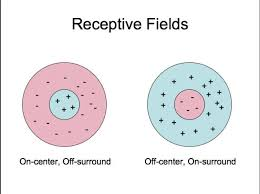
\includegraphics[width=6cm]{images/rf.jpg}
\caption{Receptive Field}
\label{fig: RF}
\end{figure}

\textbf{Optic Chiasm:} after exiting the eye and traveling along the optic nerve, the optic nervs of each eye intersect. (named after the Greek letter \textit{chi}, which looks like an X representing the crossing) \\

At the cross the fibers from the two optic nerves divide into two new groups, with axons from each of the eyes that gather information from the left visual field going to the right half of the brain and and the right visual field going to the left half of the brain. \\

About 10\% of the optic nerve axons go into part of the midbrain called the \textit{superior colliculus}. \\

\noindent \textbf{Superior colliculus:} heavily involved in very rapid responses to sensory stimuli in ways that do not involve awareness.\\
You notice something in the periphery of your visual field and begin to turn toward it to get a better look, before you are even aware you saw anything. \\

Almost 90\% of the optic nerve axons head to the \textit{thalamus} in the diencephalon, where they enter a pair of  structures called the \textbf{lateral geniculate nuclei}. \\

LGN sends information to the \textbf{posterior occipital lobe} or the \textbf{visual cortex (V1)} \\

\noindent \textbf{Contralateral Connectivity:} Crossing over of information between the spatial environment and the brain (note visual field not eyeballs)\\
\noindent \textbf{Left} Visual Field $\rightarrow$ \textbf{Right} LGN $\rightarrow$ \textbf{Right} Occipital Lobe\\
\textbf{Right} Visual Field $\rightarrow$ \textbf{Left} LGN $\rightarrow$ \textbf{Left} Occipital Lobe \\

\subsection{Visual Cortex}
Occipital lobes, together with posterior regions of the temporal lobes (LGN), are involved in the analysis of visual information. \\

From LGN, information goes to part of the posterior occipital lobe known as visual area 1 (V1). Cells in V1 send axons to nearby regions of the cerebral cortex called V2, V3, V4, V5. \\
Visual Properties: 
\begin{itemize}
    \item V1: visual stimuli having edge of contrast oriented in space may be used to construct the overall shape of an object (simple cells, complex cells, hypercomplex cells) 
    \item V4: Responds to specific colors and are less influenced by things like shape and movement (ventral stream / temporal area) 
    \item V5: Responds to movement and its speed and direction and are not so influenced by things like shape and color (dorsal stream / parietal area / somatosensory cortex) 
\end{itemize}

Topographic maps are preserved throughout the visual areas meaning that objects in space that trigger photoreceptors in a specific area of the retina will respond to the same area in the LGN and Visual Cortex. \\

Most of what we know about the visual system, through the studying of animals brains and visual stimuli, has been discovered by David Hubel and Torsten Wiesel. \\

\newpage
\section{Visual Disabilities}

\noindent \textbf{Visual Scotoma:} a blind spot in a specific region of space (caused by a lesion or damage to V1). V1 is important to flow of information in brain. \\

\noindent \textbf{Heminaopsia:} loss of vision in one half of visual space. \\

\noindent \textbf{Cortical Achromatopsia:} disruption of color vision. (due to damage of V4) (cortical because it is related to cortical lesion) \\

\noindent \textbf{Akinetopsia:} motion blindness, person becomes unaware of movement in some region of visual space. World appears as series of snapshots. (due to lesion in V5) \\

\noindent \textbf{Prosopagnosia:} face blindness, difficulty or even complete inability to recognize faces. (located in inferior(lower) and medial(middle) temporal lobe) \\

\noindent \textbf{Agnosia:} without knowledge, not knowing. \\

Persons suffering from a visual agnosia may have difficulty recognizing all or nearly all visual objects. Can identify visual scene but integrating the details into a meaningful whole object or scene difficult. Often associated with lesions in the region where the occipital, temporal and parietal lobes come together. 

\end{document}